\documentclass[11pt]{scrartcl}
\usepackage{amsmath}
\usepackage[sexy,mdthm,secthm]{evan}
\usepackage[margins=1.0in]{geometry}
\usepackage{amssymb}
\usepackage[utf8]{inputenc}

\newcommand{\p}[2]{\frac{\partial {#1}}{\partial {#2}}}
\newcommand{\inv}[1]{\frac{1}{#1}}
\newcommand{\fl}[1]{\lfloor #1\rfloor}
\newcommand{\cl}[1]{\lceil #1\rceil}

%fix margins
\usepackage[letterpaper,top=2cm,bottom=2cm,left=3cm,right=3cm,marginparwidth=1.75cm]{geometry}


\setlength{\parskip}{\baselineskip}%
\setlength{\parindent}{0pt}%
\usepackage{mathtools}
\usepackage{amssymb}
\usepackage{amsfonts}
\newcommand*\conj[1]{\bar{#1}}
\newcommand{\ord}{\text{ord}}
\newcommand{\T}{\textbf{T}}
\newcommand{\H}{\textbf{H}}
\documentclass{article}
\usepackage[utf8]{inputenc}
\usepackage[dvipsnames]{xcolor} % let LaTeX work with colors
\usepackage{framed} % useful for creating "boxes"

\colorlet{shadecolor}{orange!15} % I like orange-colored boxes.

\usepackage{amsthm}


\title{Latex Testing}
\author{Ryan Yang}
\date{April 2021}

\begin{document}

\maketitle



\begin{theorem}
pog
\end{theorem}

\begin{claim}
almost as pog
\end{claim}

\begin{lemma}
lemme in
\end{lemma}



\section{Problem Statement}
\begin{problem}
\[\text{Evaluate} \lim_{x \to +\infty} \frac{x^{1000}-1}{x-1}\]
\end{problem}

\begin{proof}
\[\lim_{x \to +\infty} \frac{x^{1000}-1}{x-1} = \lim_{x \to +\infty} \frac{1000x^{999}}{1} = 1000 \]
\end{proof}


\[\frac{1}{kx/y+z/ky+1}+\frac{1}{ky/z+x/kz+1}+\frac{1}{kz/x+y/kx+1}\geq \frac{3^2}{3+k(x/y+y/z+z/x)+1/k (z/y+x/z+y/x)))}\]

\[\frac{ky^2}{k^2xy+ky^2+yz}+\frac{kz^2}{k^2yz+kz^2+xz}+\frac{kx^2}{k^2xz+kx^2+xy}\]
By titu's,
\[\geq \frac{k(x+y+z)^2}{k^2(xy+yz+xz)+k(y^2+x^2+z^2)+(yz+xz+xy)}\]
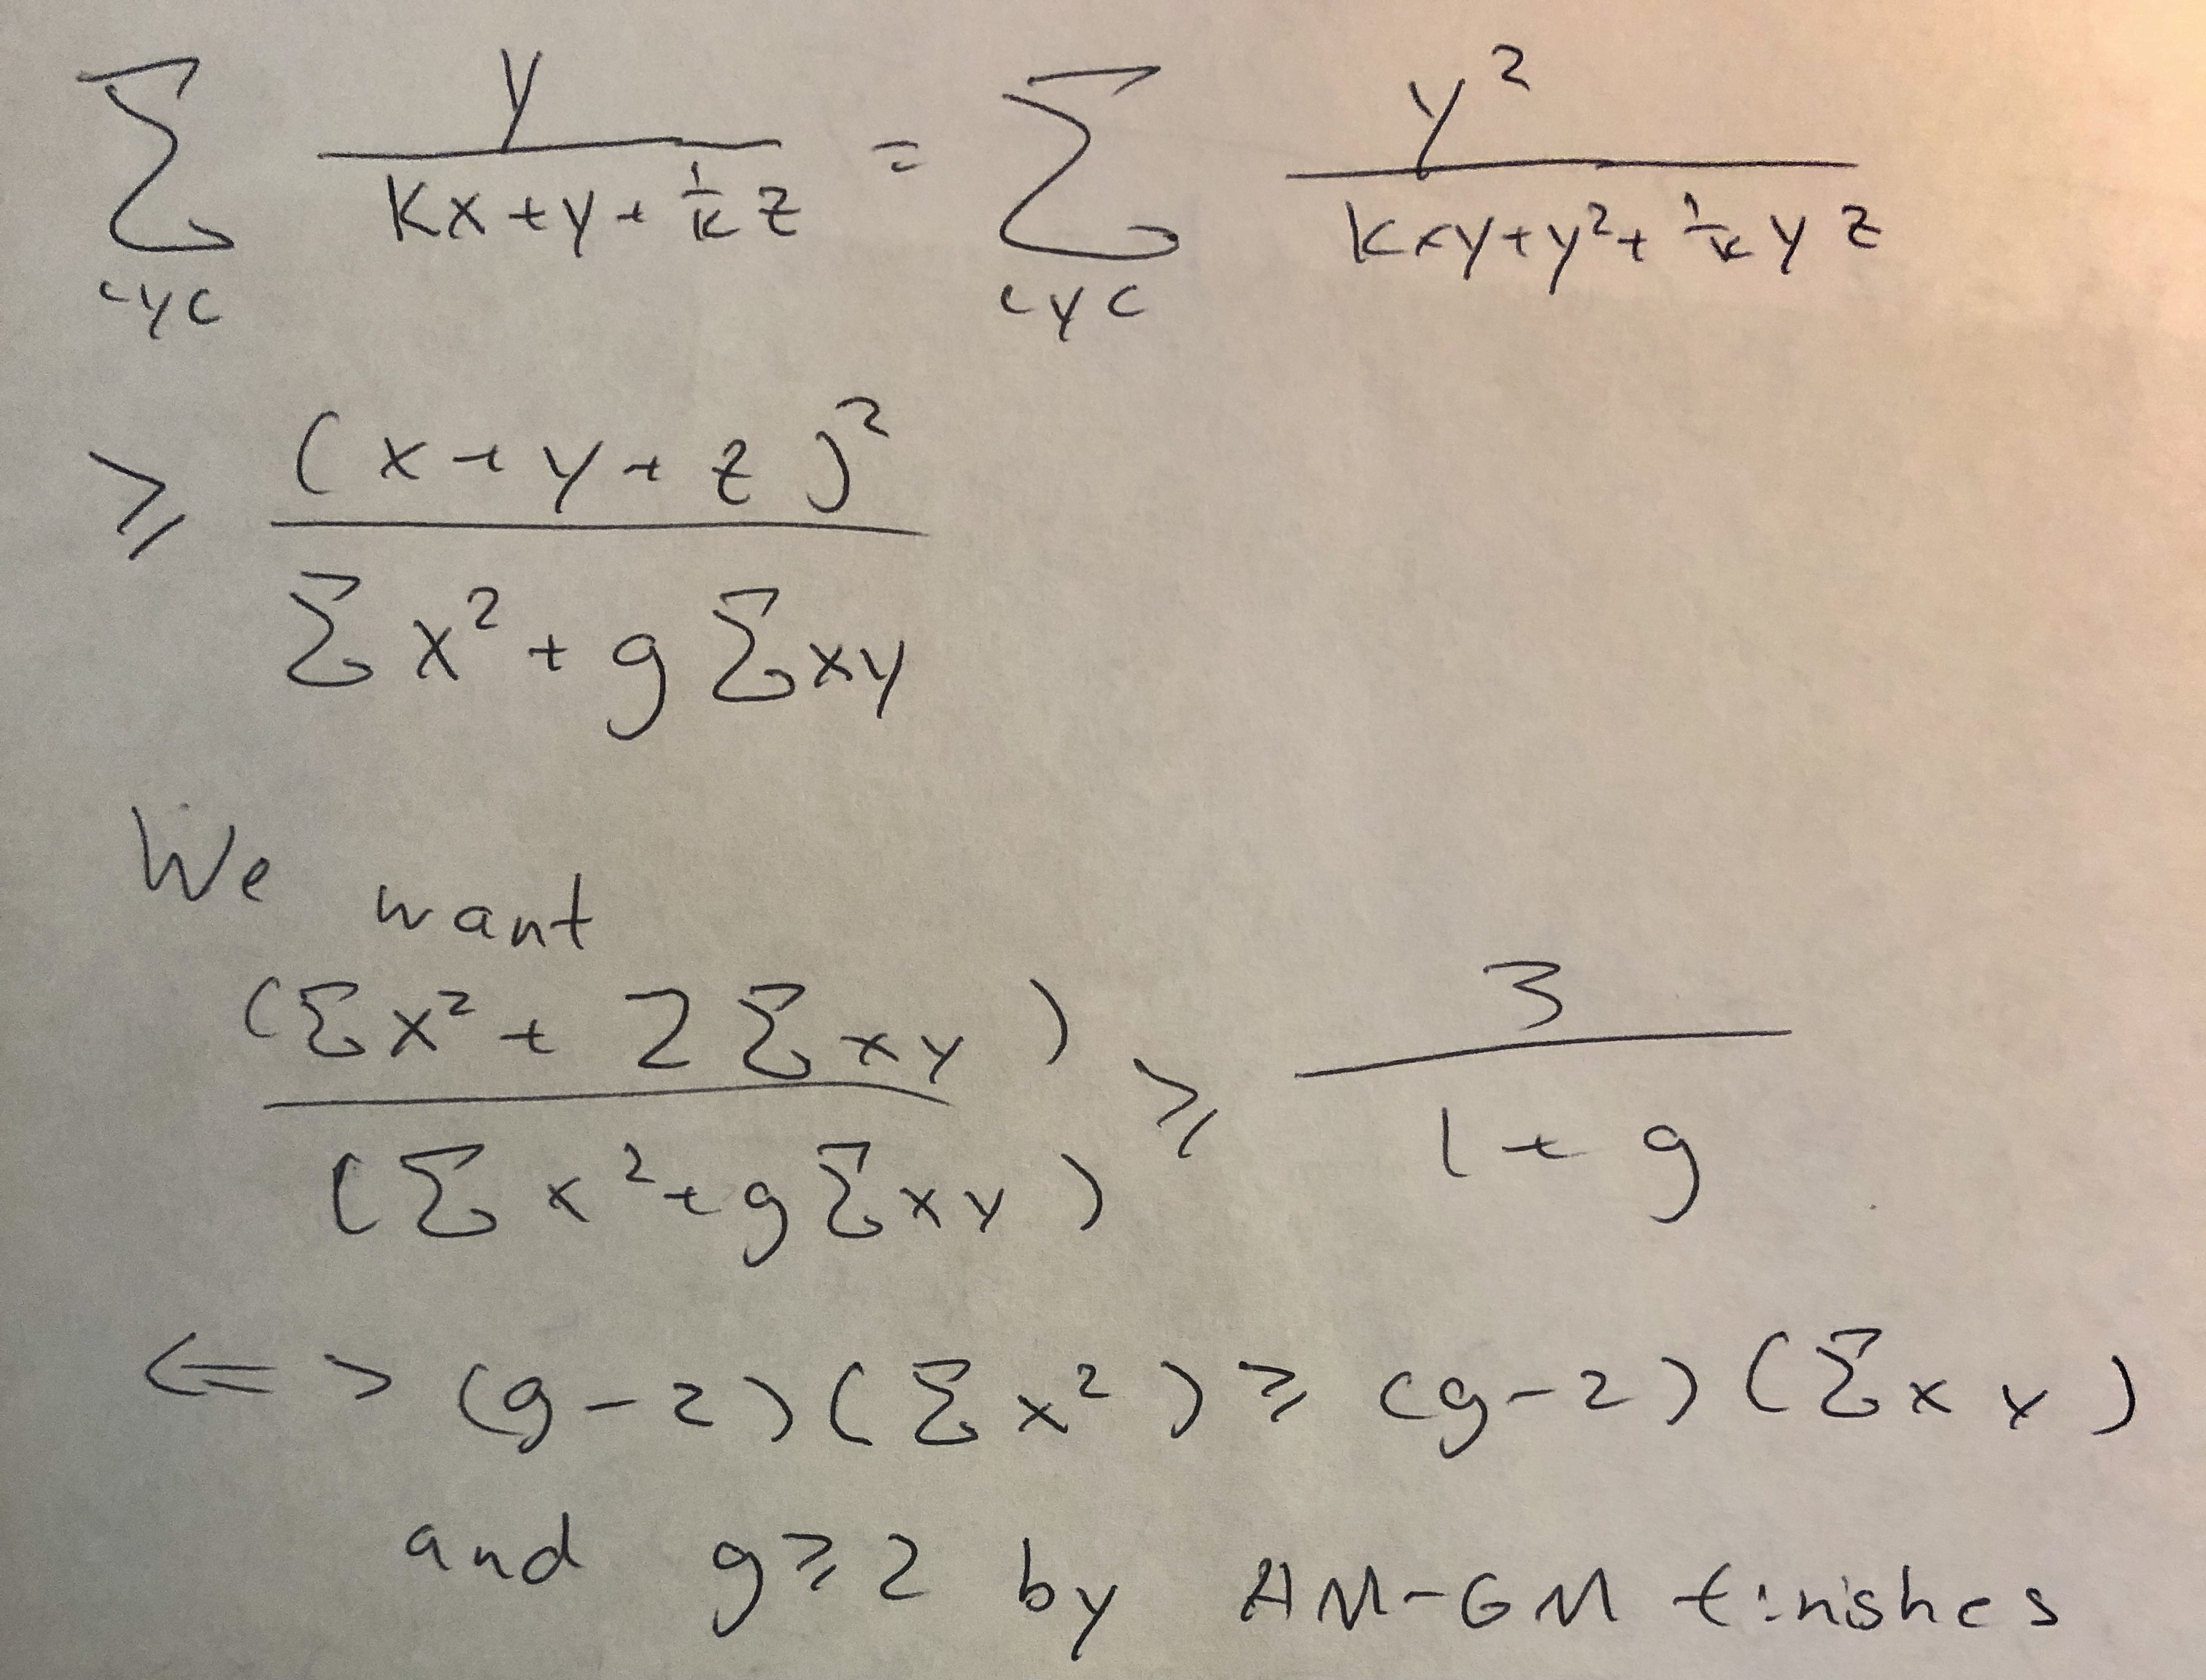
\includegraphics[scale=0.1]{huh-a2.jpg}
\end{document}
